\documentclass[12pt,a4paper]{article}

\usepackage[utf8]{inputenc}
\usepackage[T2A]{fontenc}
\usepackage[ukrainian]{babel}
\usepackage{float}  % в преамбулі
\usepackage{graphicx}
\usepackage{subcaption}  % середовище subfigure
\usepackage{amsmath, amssymb}

\usepackage{geometry}
\geometry{
    left=2cm,
    right=2cm,
    top=2cm,
    bottom=2cm
}

\begin{document}

    \begin{titlepage}

        \thispagestyle{empty}
        \begin{center}
        \large
        Національний технічний університет України\\
        «Київський політехнічний інститут імені Ігоря Сікорського»\\[1em]
        Факультет інформатики та обчислювальної техніки\\
        Кафедра обчислювальної техніки
        \end{center}

        \vfill

        \begin{center}
        \textbf{\LARGE Дискретна математика}\\[2em]
        \textbf{\Large Лабораторна робота №5}\\
        «Комбінаторика: перестановки, розміщення, сполучення» 
        \end{center}

        \vfill

        \begin{flushright}
        Виконав: студент 1 курсу ФІОТ, гр. ІО-41\\
        \textit{Давидчук А. М.}\\
        Залікова книжка № 4106\\[1em]
        Перевірив: \textit{Пономаренко А.\,М.}
        \end{flushright}

        \vfill

        \begin{center}
        Київ -- 2025
        \end{center}

    \end{titlepage}

    \setlength{\parindent}{0pt}

    \textbf{\underline{Тема:}} «Комбінаторика: перестановки, розміщення, сполучення».

    \vspace{1em}

    \textbf{\underline{Мета:}}
    вивчення правил утворення комбінацій множин: \textit{перестановок}, \textit{розміщень}, \textit{сполучень}.

    \vspace{1em}

    \textbf{\underline{Короткі теоретичні відомості:}}

    \vspace{1em}

    \textbf{Множина} --- це сукупність елементів, що задовольняють певній властивості. Елементи множини можуть бути будь-якими об’єктами (числа, кортежі, символи тощо). Якщо всі елементи однієї множини належать іншій, то перша множина називається \textbf{підмножиною} другої.

    \vspace{1em}

    \textbf{Кортеж} --- впорядкована структура фіксованої довжини. У лабораторній використовуються кортежі з двох компонент: ім’я (рядок) та вік (ціле число).

    \vspace{1em}

    \textbf{Сортування} --- це впорядкування елементів множини за зростанням або спаданням згідно з певним критерієм. Серед відомих методів сортування виділяється алгоритм \textbf{швидкого сортування (QuickSort)}, який реалізує підхід ``розділяй і володарюй''. Він вибирає опорний елемент (pivot), ділить масив на менші та більші за pivot підмасиви й рекурсивно їх сортує. Середня складність алгоритму — $O(n \log n)$, найгірший випадок — $O(n^2)$.

    \vspace{1em}

    \textbf{Пошук} --- це операція визначення наявності елемента у множині. У відсортованих масивах ефективним є \textbf{двійковий пошук (binary search)}, що ділить масив навпіл, порівнює середину з цільовим значенням і рекурсивно чи ітеративно звужує діапазон. Має логарифмічну складність $O(\log n)$.

    \vspace{1em}

    \textbf{Фільтрація множини} --- це процес побудови підмножини з елементів, що задовольняють задану умову. У даному випадку критерієм є належність віку до деякого набору.

    \vspace{1em}

    \textbf{Композиція алгоритмів} дозволяє поєднати сортування та пошук для оптимального вибору підмножини. Спочатку вся множина впорядковується за віком (QuickSort), далі для кожного віку, вказаного користувачем, виконується двійковий пошук усіх відповідних елементів. Такий підхід ефективний навіть для великих обсягів даних.

    \vspace{2em}

    \textbf{\underline{Завдання за варіантом:}} $4106$ mod $26 + 1 = 25$:

    \begin{figure}[ht]
        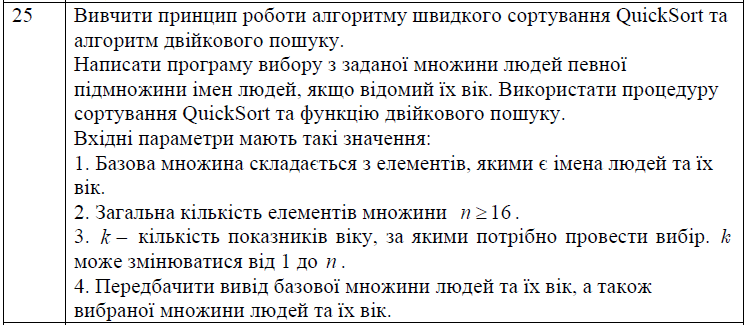
\includegraphics[width=1.0\textwidth]{photo1.png}
    \end{figure}

    \setlength{\parindent}{0pt}

    Блок-схеми алгоритму швидкого сортування (\texttt{qsort}) та двійкового пошуку (\texttt{binsearch}):

    \begin{figure}[H]
        %--- верхній ряд ---
        \begin{subfigure}{0.23\textwidth}
            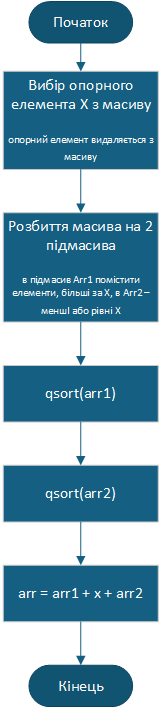
\includegraphics[width=\linewidth]{arg_qsort.png}
            \label{fig:a}
        \end{subfigure}
        \begin{subfigure}{0.76\textwidth}
            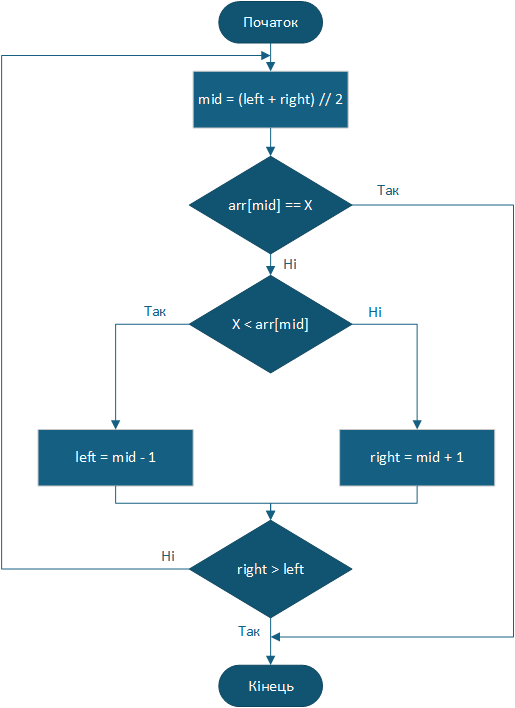
\includegraphics[width=\linewidth]{bin_sort.png}
            \label{fig:b}
        \end{subfigure}
    \end{figure}

    \newpage

    \textbf{\underline{Код:}}

    \vspace{1em}

    {

    \begin{verbatim}
import tkinter as tk
from tkinter import messagebox

def quicksort(arr):

    if len(arr) <= 1: return arr

    pivot = arr[0][1]
    less = [x for x in arr[1:] if x[1] <= pivot]
    greater = [x for x in arr[1:] if x[1] > pivot]

    return quicksort(less) + [arr[0]] + quicksort(greater)

def binary_search(arr, target):

    result = []
    left, right = 0, len(arr) - 1

    while left <= right:
    
        mid = (left + right) // 2
        age = arr[mid][1]

        if age == target:

            i = mid
            while i >= 0 and arr[i][1] == target:
                result.append(arr[i])
                i -= 1
            i = mid + 1
            while i < len(arr) and arr[i][1] == target:
                result.append(arr[i])
                i += 1
            break

        elif age < target: left = mid + 1
        else: right = mid - 1

    return result

people = [
    ("Анна", 20), ("Ігор", 25), ("Оля", 20), ("Сергій", 30), ("Марія", 25),
    ("Петро", 18), ("Люда", 22), ("Василь", 30), ("Катя", 19), ("Максим", 20),
    ("Олексій", 24), ("Даша", 21), ("Яна", 23), ("Тарас", 30), ("Інна", 19),
    ("Микола", 25), ("Юля", 16), ("Ростик", 17), ("Олеся", 17), ("Богдан", 31),
    ("Олена", 35), ("Роман", 40), ("Артем", 18), ("Михайло", 19),("Едуард", 7)
]

sorted_people = quicksort(people)

root = tk.Tk()
root.title("Вибір імен за віком")
root.resizable(False, False)

base_label = tk.Label(root, text="Базова множина (Ім'я - Вік):")
base_label.pack()

base_text = tk.Text(root, height=10, width=40)
for name, age in sorted_people:
    base_text.insert(tk.END, f"{name} - {age} років\n")
base_text.config(state=tk.DISABLED)
base_text.pack()

entry_label = tk.Label(root, text="Введіть потрібні віки через кому:")
entry_label.pack()

entry = tk.Entry(root, width=30)
entry.pack()

result_label = tk.Label(root, text="Підмножина імен:")
result_label.pack()

result_text = tk.Text(root, height=5, width=40)
result_text.config(state=tk.DISABLED)
result_text.pack()

def search():

    input_str = entry.get()

    try: target_ages = list(map(int, input_str.split(",")))

    except ValueError:
        messagebox.showerror("Помилка", "Введіть числа, розділені комами")
        return

    names = []
    for age in target_ages:
        matches = binary_search(sorted_people, age)
        names.extend([name for name, _ in matches])

    result_text.config(state=tk.NORMAL)
    result_text.delete(1.0, tk.END)

    if names:
        for name in names: result_text.insert(tk.END, name + "\n")
    else: result_text.insert(tk.END, "Нічого не знайдено")

    result_text.config(state=tk.DISABLED)

button = tk.Button(root, text="Знайти імена", command=search)
button.pack(pady=5)

root.mainloop()
    \end{verbatim}
}

    \textbf{\underline{Скріншоти виконання програми:}}

    \begin{figure}[htbp]
        %--- верхній ряд ---
        \begin{subfigure}{0.33\textwidth}
            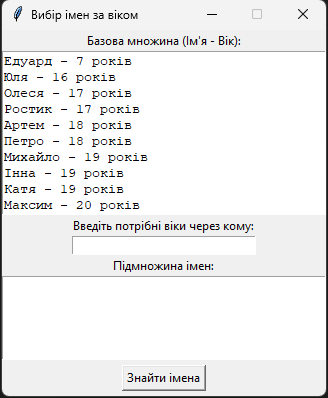
\includegraphics[width=\linewidth]{ex0.png}
            \label{fig1:a}
        \end{subfigure}
        \begin{subfigure}{0.33\textwidth}
            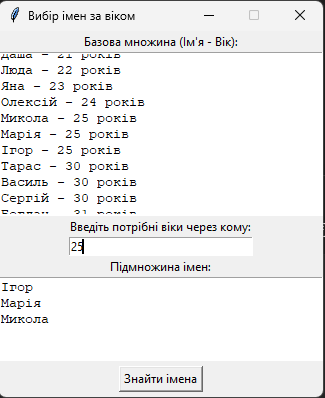
\includegraphics[width=\linewidth]{ex1.png}
            \label{fig1:b}
        \end{subfigure}

        %--- нижній ряд ---
        \begin{subfigure}{0.33\textwidth}
            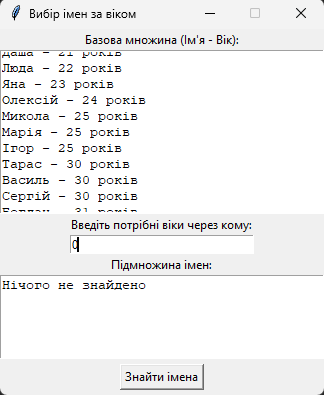
\includegraphics[width=\linewidth]{ex2.png}
            \label{fig1:c}
        \end{subfigure}
        \begin{subfigure}{0.33\textwidth}
            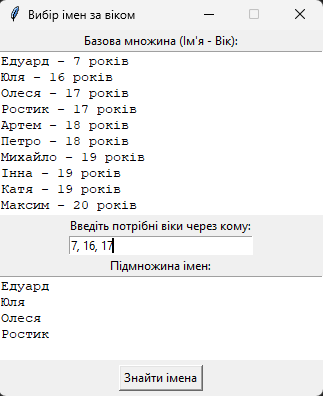
\includegraphics[width=\linewidth]{ex3.png}
            \label{fig1:d}
        \end{subfigure}

        \label{fig1:grid4}
    \end{figure}

    \textbf{\underline{Висновок:}}
    Під час лабораторної роботи  було розроблено графічну програму на мові Python з бібліотекою \texttt{tkinter}, яка дозволяє користувачам фільтрувати людей за віком. З цієї причини підхід до програмування був заснований на загальних алгоритмах: QuickSort для впорядкування набору за віком та Binary Search для швидкого пошуку певних вікових рівнів.
    Результати показують правильність обраного підходу та ілюструють, як методи програмування можуть бути реалізовані в інтерактивних інструментах.

\end{document}